\whiteBGstarBegin
\setcounter{section}{0}
\section{Trắc nghiệm}
\begin{enumerate}[label=\bfseries Câu \arabic*:]
	
	\item \mkstar{1}
	
	\cauhoi
	{Lực tác dụng vào vật làm cho vật quay quanh một trục có giá
		\begin{mcq}
			\item song song với trục quay.
			\item cắt trục quay.
			\item nằm trong mặt phẳng song song với trục quay.
			\item nằm trong mặt phẳng vuông góc với trục quay và không cắt trục quay.
		\end{mcq}
	}
	
	\loigiai
	{	\textbf{Đáp án: D.}
		
		Lực tác dụng vào vật làm cho vật quay quanh một trục có giá nằm trong mặt phẳng vuông góc với trục quay và không cắt trục quay.
	}
	
	\item \mkstar{2}
	
	\cauhoi
	{Một thanh AB có chiều dài $\text{AB} = \SI{7.5}{m}$ có trọng lượng $\SI{200}{N}$ có trọng tâm G cách đầu A một đoạn $\SI{2}{m}$. Thanh có thể quay xung quanh một trục đi qua O. Biết $\text{OA} = \SI{2.5}{m}$. Để thanh AB nằm cân bằng, phải tác dụng vào đầu B một lực $F$ có độ lớn bằng
		\begin{mcq}(4)
			\item $\SI{100}{N}$.
			\item $\SI{25}{N}$.
			\item $\SI{10}{N}$.
			\item $\SI{20}{N}$.
		\end{mcq}
	}
	
	\loigiai
	{	\textbf{Đáp án: D.}
		
	Chọn trục quay qua O. Theo quy tắc momen lực:
	$$P \cdot \text{OG} = F \cdot \text{OB} \Rightarrow F =\dfrac{\SI{200}{N} \cdot \SI{0.5}{m}}{\SI{5}{m}}= \SI{20}{N}$$
	
	}
	\item \mkstar{3}
	
	\cauhoi
	{Một thanh nhẹ gắn vào sàn tại B như hình vẽ.
		\begin{center}
			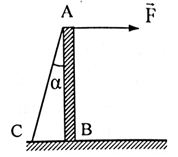
\includegraphics[scale=1]{../figs/VN10-2021-PH-TP021-6.png}
		\end{center}
	Tác dụng lên đầu A lực kéo $F=\SI{100}{N}$ theo phương ngang. Thanh được giữ cân bằng nhờ dây AC. Lực căng của dây có giá trị là bao nhiêu? Biết $\alpha = 30^\circ$.
		\begin{mcq}(4)
			\item $\SI{250}{N}$.
			\item $\SI{150}{N}$.
			\item $\SI{100}{N}$.
			\item $\SI{200}{N}$.
		\end{mcq}
	}
	
	\loigiai
	{	\textbf{Đáp án: D.}	
		
	Chọn trục quay tại B. Áp dụng quy tắc momen lực:
	$$F \cdot \text{AB} = T \cdot \text{AB} \cdot \sin \alpha \Rightarrow T = \dfrac{F}{\sin \alpha} = \SI{200}{N}$$
	}
	
	
	
	\item \mkstar{4}
	
	\cauhoi
	{Bán cầu đồng chất khối lượng $\SI{100}{g}$. Trên mép bán cầu đặt một vật nhỏ khối lượng $\SI{7.5}{g}$. Hỏi mặt phẳng của bán cầu sẽ nghiêng góc $\alpha$ bao nhiêu khi nó cân bằng? Biết rằng trọng tâm bán cầu cách mặt phẳng của bán cầu một đoạn $3R/8$ (với $R$ là bán kính của bán cầu).
		\begin{center}
			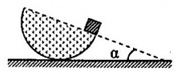
\includegraphics[scale=1]{../figs/VN10-2021-PH-TP021-7.png}
		\end{center}
		\begin{mcq}(4)
			\item $11,31^\circ$.
			\item $15^\circ$.
			\item $20^\circ$.
			\item $12^\circ$.
		\end{mcq}
	}
	
	\loigiai
	{	\textbf{Đáp án: A.}
		
				\begin{center}
			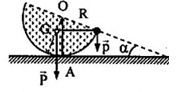
\includegraphics[scale=1]{../figs/VN10-2021-PH-TP021-8.png}
		\end{center}
	
	Các lực tác dụng lên bán cầu: trọng lực $\vec P$ của bán cầu, trọng lực $\vec p$ của vật nhỏ, phản lực $\vec Q$ tại điểm tiếp xúc A.
	
	Áp dụng quy tắc momen lực với trục quay qua O:
	$$P \cdot \text{OG} \cdot \sin \alpha = p \cdot R \cdot \cos \alpha \Rightarrow \tan \alpha = \dfrac{8m}{3M} \Rightarrow \alpha = 11,31^\circ$$
	}
	
	\item \mkstar{4}
	
	\cauhoi
	{Gió thổi vào xe theo hướng vuông góc với thành bên của xe với vận tốc $V$. Xe có khối lượng $m=\SI{e4}{kg}$, chiều cao $2b=\SI{2.4}{m}$, chiều ngang $2a=\SI{2}{m}$, chiều dài $l=\SI{8}{m}$. Áp suất gió tính bởi công thức $p=\rho V^2$, với $\rho = \SI{1.3}{kg/m^3}$ là khối lượng riêng của không khí. Vận tốc gió phải thỏa mãn điều kiện như thế nào thì sẽ khiến xe bị lật ngã?
		\begin{mcq}(2)
			\item $V \geq \SI{32}{m/s}$.
			\item $V \geq \SI{58}{m/s}$.
			\item $V \geq \SI{42}{m/s}$.
			\item $V \geq \SI{28}{m/s}$.
		\end{mcq}
	}
	
	\loigiai
	{	\textbf{Đáp án: B.}
	
	Áp dụng công thức tính áp suất:
	$$F=pS = \rho V^2 S = \rho V^2 2bl$$
		
	Các lực tác dụng lên xe: trọng lực $\vec P$, phản lực $\vec Q$, lực tác dụng $\vec F$ của gió.
	
	Khi xe bắt đầu lật, theo quy tắc momen lực đối với trục qua hai bánh xe:
	$$mg \cdot a = F \cdot b \Rightarrow V = \dfrac{1}{b} \sqrt{\dfrac{amg}{2\rho l}} \approx \SI{57.8}{m/s} $$
	
	Vậy điều kiện về vận tốc gió để khiến xe bị lật ngã là $V \geq \SI{58}{m/s}$.
	}
	
\end{enumerate}

\whiteBGstarEnd

\loigiai
{
	\begin{center}
		\textbf{BẢNG ĐÁP ÁN}
	\end{center}
	\begin{center}
		\begin{tabular}{|m{2.8em}|m{2.8em}|m{2.8em}|m{2.8em}|m{2.8em}|m{2.8em}|m{2.8em}|m{2.8em}|m{2.8em}|m{2.8em}|}
			\hline
			1.D  & 2.D  & 3.D  & 4.A  & 5.B  & & & & &  \\
			\hline
			
		\end{tabular}
	\end{center}
}
\section{Tự luận}
\begin{enumerate}[label=\bfseries Câu \arabic*:]
	\item \mkstar{1}
	
	\cauhoi{
		Momen lực đối với một trục quay là gì? Phát biểu điều kiện cân bằng của một vật có trục quay cố định (hay quy tắc momen lực).
	}
	
	\loigiai{
		Momen lực đối với một trục quay là đại lượng đặc trưng cho tác dụng làm quay của lực và được đo bằng tích của lực với cánh tay đòn của nó.
		$$M=Fd,$$
		trong đó:
		\begin{itemize}
			\item $F$ là lực tác dụng $(\SI{}{N})$;
			\item $d$ là cánh tay đòn (là khoảng cách từ giá của lực đến trục quay) $\SI{}{m}$.
		\end{itemize}
		
		Muốn một vật có trục quay cố định nằm cân bằng thì tổng các momen lực có xu hướng làm cho vật quay theo chiều kim đồng hồ phải bằng tổng các momen lực có xu hướng làm cho vật quay ngược chiều kim đồng hồ.
	}
	
	\item \mkstar{2}
	
	\cauhoi
	{Hãy giải thích hoạt động của chiếc cân (hình vẽ).
		\begin{center}
			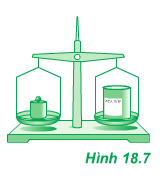
\includegraphics[scale=1]{../figs/VN10-2021-PH-TP021-5.png}
		\end{center}
	}
	
	\loigiai
	{
		Khi cân nằm cân bằng (kim chỉ thẳng đứng), theo quy tắc momen lực, ta có:
		$$P_\text{vật} d_1 = P_\text{cân} d_2$$
		
		Vì $d_1=d_2$ nên khi đó $P_\text{vật} = P_\text{cân}$. Suy ra khối lượng vật cần đo bằng khối lượng của quả cân.
		
	Cân hoạt động theo quy tắc momen lực.
	}
	\item \mkstar{3}
	
	\cauhoi
	{Một người dùng búa để nhổ một chiếc đinh, khi người đó tác dụng một lực $\SI{50}{N}$ vào đầu búa thì đinh bắt chuyển động. Biết cánh tay đòn của lực tác dụng của người đó là $\SI{20}{cm}$ và cánh tay đòn của lực nhổ đinh khỏi gỗ là $\SI{2}{cm}$. Hãy tính lực cản của gỗ tác dụng vào đinh.
	}
	
	\loigiai
	{Gọi 
		\begin{itemize}
			\item $M_1$ và $M_2$ là momen lực do tay người và lực cản của gỗ tác dụng lên búa ($\textrm{Nm}$),
			\item $F_1$ là lực do tay người tác dụng vào đầu búa ($\textrm{N}$),
			\item $F_2$ là lực nhổ đinh, hay là lực cản của gỗ cây đinh lại ($\textrm{N}$), 
			\item  $d_1=\SI{20}{cm}$ là cánh tay đòn từ tay người đến trục quay ($\textrm{m}$), 
			\item  $d_2=\SI{2}{cm}$ là cánh tay đòn từ đinh đến trục quay ($\textrm{m}$). 
		\end{itemize}
		
		Khi đinh bắt đầu chuyển động, câu búa đang ở trạng thái cân bằng, nên ta áp dụng quy tắc momen lực
		%
		\begin{equation*}
			M_1=M_2 \Rightarrow F_1\cdot d_1 = F_2\cdot d_2
		\end{equation*}
		% 
		Từ đó, ta tính được lực cản của gỗ tác dụng vào đinh 
		%
		\begin{equation*}
			F_2=F_2\cdot \dfrac{d_1}{d_2}
			=
			\SI{50}{N}\cdot \dfrac{\SI{20}{cm}}{\SI{2}{cm}}
			=
			\SI{500}{N}.
		\end{equation*}
		%
		Vậy lực cản do miếng gỗ tác dụng lên cây đinh lúc đó là $F_2=\SI{500}{N}$.
	}
	\item \mkstar{4}
	
	\cauhoi
	{Một thanh gỗ dài $\SI{1,8}{m}$ nặng $\SI{30}{kg}$, một đầu được gắn vào trần nhà nhờ một bản lề, đầu còn lại được buộc vào một sợi dây và gắn vào trần nhà sao cho phương của sợi dây thẳng đứng và giữ cho tấm gỗ nằm nghiêng hợp với trần nhà nằm ngang một góc $45^{\circ}$. Biết trọng tâm của thanh gỗ cách đầu gắn sợi dây $\SI{60}{cm}$. Tính lực căng của sợi dây, lấy $g=\SI[parse-numbers=false]{10}{m/s^2}$.
		\begin{center}
			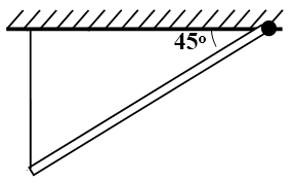
\includegraphics[scale=0.7]{../figs/VN10-2021-PH-TP021-1.png}
		\end{center} 
	}
	
	\loigiai
	{Đầu tiên, ta quy định các đại lượng trong bài toán và xác định cánh tay đòn như sau: 
		\begin{itemize}
			\item $T$ là lực căng của sợi dây tác dụng lên điểm A trên tấm gỗ, 
			\item $P=m\cdot g= \SI{30}{kg} = \SI{300}{N}$ là trọng lực tác dụng lên tấm gỗ tại trọng tâm G, 
			\item $\alpha = 45^{\circ}$ là góc hợp bởi tấm gỗ và trần nhà, 
			\item $d$ là khoảng cách từ điểm G đến trục quay O,
			\item $d'$ là khoảng cách từ điểm treo của dây đến trục quay O,
			\item $l=\SI{1,8}{m}$ là chiều dài của thanh gỗ. 
		\end{itemize}
		%--------------------------------%
		\begin{center}
			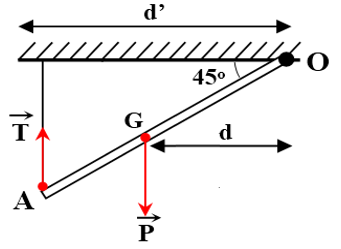
\includegraphics[scale=0.7]{../figs/VN10-2021-PH-TP021-2.png}
		\end{center}
		Tiếp theo, ta tính độ dài các cánh tay đòn bằng cách áp dụng công thức \eqref{ctd}. Cánh tay đòn của trọng lực là
		\begin{equation*}
			d=\textrm{OG}\cdot\cos 45^{\circ}=\dfrac{1}{2}\cdot \SI{1,8}{m}\cdot \cos 45^{\circ}.
		\end{equation*}
		%
		Cánh tay đòn tương ứng với lực căng dây là
		\begin{equation*}
			d' = \textrm{OA}\cdot \cos 45^{\circ} =\SI{1,8}{m}\cdot \cos 45^{\circ}.
		\end{equation*}
		%
		Áp dụng quy tắc momen lực, ta có
		\begin{align*}
			T\cdot d' &= P\cdot d\\
			\Rightarrow
			T&=\dfrac{P\cdot d}{ d'}
			=
			\dfrac{\SI{300}{N}\cdot \dfrac{1}{2}\cdot \SI{1,8}{m}\cdot \cos 45^{\circ}}{\SI{1,8}{m}\cdot \cos 45^{\circ}}
			=\SI{150}{N}
		\end{align*}
		Vậy lực căng dây là $T=\SI{150}{N}$. 
	}
	\item \mkstar{4}
	
	\cauhoi
	{Thanh OA có khối lượng không đáng kể, có chiều dài $\SI{20}{cm}$, quay dễ dàng quanh trục nằm ngang O. Một lò xo gắn vào điểm giữa C. Người ta tác dụng vào đầu A của thanh một lực $F=\SI{200}{N}$ hướng thẳng đứng xuống dưới. Khi thanh ở trạng thái cân bằng, lò xo có hướng vuông góc với OA, và OA hợp với đường thẳng nằm ngang một góc $\alpha=30^{\circ}$. Tìm phản lực N của lò xo lên thanh. 
		%%%%
		\begin{center}
			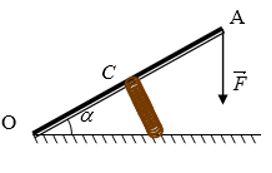
\includegraphics[scale=1]{../figs/VN10-2021-PH-TP021-3.png}
		\end{center}
	}
	
	\loigiai
	{Đầu tiên, ta xác định các cánh tay đòn của phản lực $N$ và lực $F$. Cánh tay đòn của lực N là 
		\begin{equation*}
			\textrm{OC} = \dfrac{1}{2}\cdot \textrm{OA},
		\end{equation*}
		%
		do đoạn thẳng này vuông góc với giá của lực N. Cánh tay đòn tương ứng với lực $F$ là
		%
		\begin{equation*}
			\textrm{OB} = \textrm{OA}\cdot \cos\alpha.
		\end{equation*}
		%
		\begin{center}
			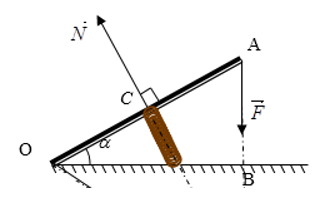
\includegraphics[scale=1]{../figs/VN10-2021-PH-TP021-4.png}
		\end{center}
		%
		Áp dụng quy tắc momen lực, ta có 
		%
		\begin{align*}
			&M_F=M_N\\
			\Rightarrow& F\cdot \textrm{OB} = N\cdot \textrm{OC}\\
			\Rightarrow& N  = \dfrac{F\cdot \textrm{OB}}{\textrm{OC}}
			=
			\dfrac{F\cdot \textrm{OA}\cdot \cos\alpha}{\dfrac{1}{2}\cdot \textrm{OA}}
			=2\cdot F\cdot \cos\alpha = \SI[parse-numbers=false]{20\sqrt{3}}{N}.
		\end{align*}
		%%%%
		Vậy phản lực tác dụng lên thanh có độ lớn là $N=\SI[parse-numbers=false]{20\sqrt{3}}{N}$
	}
\end{enumerate}